\documentclass{article}
\usepackage[left=2cm,right=2cm,top=2cm,bottom=2cm]{geometry} 
\usepackage{graphicx} 
\usepackage[spanish]{babel}
\usepackage{titlesec}
\setcounter{secnumdepth}{3}
\usepackage[section]{placeins}

%--------------------- Custom commands ------------------------------
\newcommand*\rbreak{\par\noindent\linebreak}
\newcommand*\casoheadera[2]{
	\textbf{#1} & 
	\parbox[t]{12cm}{#2} \\\hline
}
\newcommand\casoheaderb[2]{
	\multicolumn{2}{|l|}{
		\parbox[t]{15cm}{ \textbf{#1} \\ #2 \\ } 	
	} \\\hline
}
%------------------------ Constants ---------------------------------
\newcommand{\nombre}{Renato Josué Flores Pérez}
\newcommand{\carnet}{201709244}
\newcommand{\titulo}{Exámen Final}
\graphicspath{{/home/renato/latex/general/scrum/examen-final/images/}}

%------------------------ Title formating --------------------------

\author{\nombre , \carnet}
\title{\textbf{\Huge\titulo}}

%------------------------- Document --------------------------------
\begin{document}
\maketitle
\textbf{\huge{Parte A: Caso Netflix}}\rbreak
Conforme a la situación descrita en el caso y bajo
la óptica de la ingeniería de Software, analice y
diseñe el conjunto de aplicaciones de Software
que Netflix cesita, incluyendo la base de 
suscriptores, la gestión de inventarios, el software
por recomendación y los pedidos de los
clientes, para la transición hacia el modelo actual de
distribución de contenidos, cuyo servicio principal
es la distribución de contenidos audiovisuales
a través de una plataforma en línea o 
servicio de video bajo de manda por streaming. Utilice
los diagramas UML que considere oportunos para
modelar su solución, de tal manera que quede 
suficientemente claro todo el proceso de desarrollo
del software.
\section{Diagramas de casos de uso}
\begin{figure}[h]
	\centering
        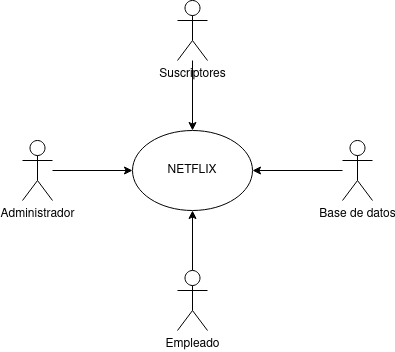
\includegraphics[width=350px,keepaspectratio]{dcu-mas-alto-nivel.png}
                 \caption{Diagrama de casos de uso de más alto nivel}
\end{figure}	

\begin{figure}[h]
	\centering
        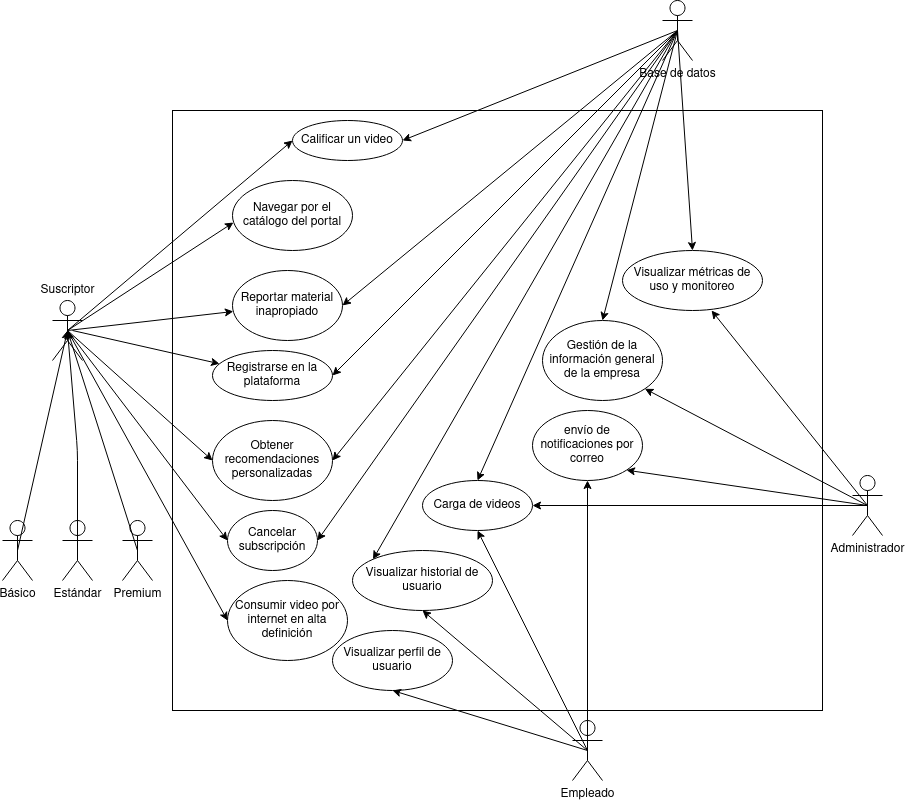
\includegraphics[width=\textwidth,keepaspectratio]{dcu-alto-nivel.png}
                 \caption{Diagrama de casos de uso de alto nivel}
\end{figure}	

\begin{figure}[h]
	\centering
        \includegraphics[width=\textwidth,keepaspectratio]{dcue-1.png}
                 \caption{diagrama de casos de uso expandido}
\end{figure}	

\begin{figure}[h]
	\centering
        \includegraphics[width=\textwidth,keepaspectratio]{dcue-2.png}
                 \caption{diagrama de casos de uso expandido}
\end{figure}	

\begin{figure}[h]
	\centering
        \includegraphics[width=\textwidth,keepaspectratio]{dcue-3.png}
                 \caption{diagrama de casos de uso expandido}
\end{figure}	

\begin{figure}[h]
	\centering
        \includegraphics[width=\textwidth,keepaspectratio]{dcue-4.png}
                 \caption{diagrama de casos de uso expandido}
\end{figure}	
\section{Modelo conceptual}
\section{Diagramas de estados y actividades}
\section{Diagrama de componentes}
\section{Diagrama de clases}
%\section{Casos de uso}
% \subsection{} %Use case name
% ------------------ Elaborate ----------------------------
\section{Resumen}
\subsection{CDN}
CDN significa Content Delivery Network, se refiere a una red 
de servidores, generalmente distribuídos al rededor del mundo
conectados  a internet que se encargan de servir contenido
estático (imágenes, video, música, pdf, html, etc). Este tipo
de redes no implementan ninguna lógica de negocio más allá de un
sistema de seguridad para prevenir el acceso no autorizado.
Estos sistemas están especializados para servir este 
contenido priorizando la velocidad de red y estabilidad de conexión.
En el contexto de Netflix este sistema será el encargado de almacenar
la filmoteca (inventario) y de servir el material videográfico 
sobre la red a los usuarios finales. 
La carga de material videográfico a este sistema está 
fuera del alcance de este y por tanto se realiza por separado.
\subsection{Sistema de monitoreo}
Una plataforma Web para uso específico interno de Netflix. Únicamente
personal interno autorizado tendrá acceso a esta app y se trata
de un portal web que habilitará a los altos mandos de Netflix 
monitorear el desempeño de su plataforma en todo momento, obtener
reportes de errores, health checks de la infraestructura y demás
información útil para realizar tareas de monitoreo.
\subsection{Portal de administración}
Esta plataforma, a diferencia del sistema de monitoreo será utilizada
para realizar tareas propiamente de administración del sistema. En
este sistema se podrá cargar material videográfico al CDN, trackear
órdenes, revisar las suscripciones de los usuarios, editar la
misión, visión, logo y demás información a mostrar a los usuarios
finales. Este no debe ser forzosamente un portal web, otras
opciones que podrían considerarse es una aplicación de escritorio
escrita en C o un sistema basado en JavaFX.
\subsection{Portal del usuario final}
La plataforma web a la que los usuarios finales tendrán acceso y 
desde donde podrán consumir el contenido de Netflix. En este portal
pueden registrarse, iniciar sesión, revisar sus recomendaciones, 
buscar películas, consumir el material videográfico e incluso
cancelar su suscripción. Sin duda una pieza clave en el nuevo sistema
de Netflix.
\subsection{Sistema de recomendaciones}
El sistema insignia de Netflix, un sistema basado en MachineLearning
que ha sido el responsable de su posición y popularidad actual. Este
sistema debe ser refinado y mejorado de modo que pueda seguir siendo
utilizado de manera efetiva en el nuevo contexto.
\subsection{Sistema de susbcripciones}
El sistema de subscripciones es un sub sistema tipo backend
que se encarga de registrar y realizar todas las operaciones
relacionadas a las subscripciones de los clientes. Este sistema
será el único encargado de operar la base de datos donde dichas
transacciones estén registradas y únicamente expondrá una API
para la interacción con el resto de componentes del sistema Netflix.

\subsection{Requerimientos No Funcionales}
\begin{itemize}
	\item Alta disponibilidad
	\item Alta seguridad
	\item Alta tolerancia a los fallos
	\item Velocidad considerable de transmisión de datos
	\item Transacciones atómicas y rastreables
	\item Implementación de algoritmos de encriptación para el
		manejo de credenciales y demás información sensitiva de los
		clientes.
	\item El sistema cliente del usuario final debe estar 
		garantizado su correcto funcionamiento en los browsers más
		utilizados en el mercado.
\end{itemize}

\subsection{Requerimientos Funcionales}
\begin{itemize}
	\item Subir videos al CDN
	\item Visualizar el historial y perfil de un usuario 
		específico
	\item Obtener métricas en tiempo real del funcionamiento del
		sistema y su estado en cualquier momento en el tiempo t.
	\item Capacidad de registrarse en la plataforma
	\item Fácil navegación entre la biblioteca del portal de Netflix
	\item Capacidad de calificar un video
	\item Obtener recomendaciones y una landing page personalizada
		de acuerdo a los gustos del cliente.
	\item Habilidad para visualizar el material videográfico en alta
		definición desde el hogar del cliente en tiempo real.
	\item Capacidad de editar la información general de la empresa
	\item Notificar por correo  a los usuarios de sus 
		actividades pertinentes a su subscripcion.
\end{itemize}
\section{Tomando en cuenta la competencia y demanda de servicio,
      qué metodología de desarrollo de software adoptaría
      y por qué.}
\subsection{AUP}
Tomando en cunta la competencia, la demanda de servicio, y la 
posición actual de Netflix, la metodología de desarrollo de software 
que debería adoptarse es AUP (Agile Unified Process). \\
En vista de los antecedentes, realizar una transición 
desde un sistema de alquiler de vídeos en línea a un sistema de
consumo de video a solicitud (Streaming) es sin duda un cambio total
de paradigma. Este cambio claramente necesitará más que grandes 
esfuerzos de ingeniería de software para lograr su implementación
exitosa.  Este cambio también debe tomar en cuenta la resistencia
al cambio que muy seguramente surgirá entre el personal
administrativo, ejecutivo y financiero. Para lograr la transición
de manera exitosa, se debe prestar especial atención al análisis
y diseño de los sistemas de software a implementar, así como de 
asegurarse que todos los departamentos de la empresa entiendan
el cambio y manejen los nuevos conceptos, de manera que 
puedan fácilmente capacitarse para el uso de las nuevas
herramientas una vez estén listas. \\
Por esta razón, se ha escogido AUP. Netflix debe encontrar un 
balance entre agilidad y planeamiento, algo que AUP sin duda ofrece.
\subsection{Planificación}
La implementación de AUP como metodología de desarrollo de
software para la correcta transición de Netflix de su modelo
de negocio actual hacia un modelo de negocio basado en Streaming
debe ser cuidadosamente planificada. A continuación se detalla la
planificación para la implementación de AUP en el contexto específico
de este caso de estudio. Se detallan las 4 fases de AUP y como 
será llevado a cabo la implementación de cada una, tomando en cuenta
la problemática, los objetivos y los antecendentes de Netflix.
\subsubsection{Inicio}
La etapa de inicio será especialmente útil para introducir el 
cambio y presentar las primeras ideas para una posible solución, su 
arquitectura y un estimado de los recursos que se necesitarán.
Estos detalles serán presentados a todos los interesados del proyecto,
asegurándose que todos los departamentos pertinentes de la empresa
(financiero, administrativo, ejecutivo) posean itempo suficiente
para evaluar, entender y resolver sus dudas en cuanto al proyecto,
el nuevo modelo de negocios y su implementación. \\
Una vez terminada esta fase, el equipo estará mucho más familiarizado
con los objetivos del proyecto, los cambios que traerá, como las
distintas áreas de la empresa serán afectadas y una idea clara
de por donde comenzar su implementación.
\subsubsection{Elaboración}
Durante la etapa de Elaboración el equipo se encargará de 
llevar a cabo el despliegue inicial de la arquitectura propuesta en 
entornos de desarrollo. Se tendrá tiempo para verificar la 
arquitectura y su viabilidad en base a hechos y experiencias reales
de su desempeño tanto por parte del equipo de desarrollo como 
de los principales interesados. Se tendrá la oportunidad de replantear
la arquitectura y realistar ajustes o realizar un total rediseño
de ser necesario en base a la retroalimentación del cliente y los
resultados obtenidos de las pruebas de desempeño y estabilidad.
Nuevamente, debido a la naturaleza innovadora del servicio a
implementar, Netflix no puede darse el lujo de equivocarse al momento
de definir la Arquitectura y desplegar un sistema que produzca
resultados subóptimos para el usuario final. Netflix no puede perder
la crédibilidad y confianza que poseen con su base de subscriptores
actual. La arquitectura escogida durante esta fase debe ser escogida
en base a considerables esfuerzos de pruebas e investigación en los
campos de redes, sistemas distribuídos, clusters y seguridad.
\\
Una vez se tenga definida la Arquitectura a implementar y configurados
los entornos de desarrollo y producción, se podrá dar inicio a la 
siguiente etapa.
\subsubsection{Construcción}
Durante esta fase el equipo de desarrollo
se encargará de escribir e implementar las distintas herramientas
de Software que se planificaron. El usuario será capaz de proveer
retroalimentación en base a cada una, se vereficará su desempeño
y corroborán su alineamiento con los objetivos del proyecto, 
su alcance y los requerimientos planteados.
\subsubsection{Transición}
Finalmente, la etapa de transición. Se realizará el despliegue del
sistema en el entorno de producción oficial. Se llevarán a cabo las
primeras capacitaciones oficiales del sistema al personal de la
empresa y se comenzarán las estrategias de marketing y distribución
para dar a conocer el nuevo sistema al usuario final.
\subsection{Notas finales}
Debido a que AUP es un método ágil, se tiene la ventaja que 
una vez finalizada la cuarta etapa, se dará comienzo a la siguiente
iteración. Se revisará el alcance y los requerimientos del proyecto,
se realizarán modificaciones de ser necesario y comenzará el
desarrollo de la siguiente versión. AUP es especialmente útil ya que
se caracteríza por poseer un tiempo considerablemente largo en 
comparación con otras metodologías ágiles para la culminación 
éxitosa de su primer iteración, en contraste el tiempo necesario 
para culminar las iteraciones siguientes es significativamente menor.
Esta propiedad es especialmente útil para Netflix, ya que gozará 
de un tiempo suficiente para plantear, planificar, diseñar y ejecutar
la implementación del nuevo servicio con el debido cuidado y 
concentración. Asegurándose de esta forma que su primer versión sea tal
cual la necesita el cliente y se alínee adecuadamente a la visión de Netflix de 
su nueva estrategia y modelo de negocio. Debido al cambio 
inminente de paradigma para el público general, Netflix debe
asegurarse que este cambio sea adoptado de la forma más gentil posible
y que los usuarios finales se sientan lo más cómodos posible ante
el cambio desde su primer impresión. Debido al contexto de Netflix,
esta primer impresión del usuario final hacia el nuevo sistema es
decisiva. En consecuencia, se justifica nuevamente la adopción de AUP
como metodología de desarrollo de software ideal para este nuevo proyecto.

\section{¿Qué momentos de crisis puede identificar y como los
prevendría?}
\subsection{Resistencia al cambio}
Uno de los riesgos más comúnes durante el proceso de implementación
de un proyecto de Software es la resistencia al cambio por parte
de algunos interesados o en ocasiones de departamentos enteros
de la empresa donde se esté llevando a cabo el proyecto. Debido
a la naturaleza innovadora del nuevo proyecto Netflix y al cambio
de paradigma que este implica, la resistencia al cambio será sin
duda un momento de crisis que deberá afrontarse. Es de vital
importancia no pasarlo por alto y estar debidamente preparados con
un plan de contingencia adecuado.
\subsubsection{Solución}
La mejor forma de solucionar este problema será por medio de 
charlas y seminarios informativos internos respecto al nuevo 
concepto de Streaming previos a la revelación del nuevo plan de
negocio. Las analogías con servicios de consumo de video similares 
como YouTube pueden ser de gran ayuda para las primeras
introducciones, listando las similitudes y 
haciendo especial énfasis en las diferencias. Además de las charlas,
seminarios y analogías, se recomienda que la explicación del nuevo
modelo de negocio sea llevado a cabo por nada más y nada menos
que el mismo Hastings, quién podrá responder todas las dudas
administrativas y financieras que podrían surgir luego de revelar
la ambisciosa propuesta. Finalmente, los diagramas de modelado
del negocio serán de gran ayuda no solamente para el equipo de 
desarrollo, si no también para los departamentos financieros,
ejecutivos y administrativos quienes podrán apreciar de una manera
más gráfica y natural el nuevo modelo de negocio. Es indispensable
que los diagramas de casos de uso y el de modelo conceptual sean 
cuidadosamente diseñados para expresar correctamente el nuevo 
modelo de negocios.

\subsection{Selección inadecuada de arquitectura}
Una selección inadecuada de arquitectura es un posible riesgo que
debe ser evitado a toda costa. Una equivación al momento de
seleccionar la arquitectura a implementar conlleva a una pérdida
de tiempo y recursos financieros altísima. Si bien es posible en 
algunos casos realizar modificaciones a la arquitectura de un 
sistema, estas son por lo general cambios mínimos, pero una 
reestructuración entera de la arquitectura es algo rara vez visto
en la práctica y comúnmente conlleva al fracaso total o parcial
del proyecto en cuestión. Este riesgo es especialmente probable
en el contexto de Netflix debido a que en aquella época las 
tecnologías de Streaming no habían madurado como ahora y aún 
se encontraban etapas experimentales o académicas. Era responsabilidad
de Netflix invertir en este campo y seleccionar una arquitectura 
adecuada por sí mismos.
\subsubsection{Solución}
La forma más adecuada de evitar este problema es no dudar en la
inversión adecuada de recursos en las ramas de investigación y 
redes. Deben contratarse investigadores altamente capacitados en 
las áreas de Ciencias de la Computación, Telecomunicaciones y 
Redes cuya único rol sea la investigación académica dedicada 
hacia las tecnologías de Streaming y que puedan proveer 
documentos de estudio y guías relevantes sobre los detalles a 
tomar en cuenta cuando 
se esté seleccionando la arquitectura de los sitemas a implementar,
prestando especial atención a temas de latencia, ruteo de paquetes,
estabilidad, disponibilidad, seguridad y costos. Estas guías podrán
ser utilizadas como base al momento de decidir la Arquitectura 
a implementar.

\subsection{Pérdida del horizonte}
Para llevar a cabo la implementación éxitosa del nuevo modelo
de negocios de Netflix, se planea la implementación de varios
sistemas de software que deberán comunicarse entre sí para formar
el sistema de Netflix en su conjunto. Debido a la cantidad
considerable de sistemas a implementar: Sistema de CDN, monitoreo,
administración, recomendaciones, suscripciones y cliente. Los
diferentes protocolos de comunicación a utilizar: AMPQ, gRPC,
HTTP, WS, RESP. Es posible que el equipo de desarrollo pierda 
el horizonte, es decir olviden los objetivos generales del proyecto
y la visión de funcionamiento de alto nivel del sistema de Netflix
como un todo.
\subsubsection{Solución}
La mejor forma de prevenir este riesgo es prestando especial 
atención a la redacción y mantenimiento de una documentación robusta
y cuidando la manera en que esta sea accesible en todo momento
tanto por el equipo de desarrollo como los interesados de la 
empresa. La documentación debe contener tanto detalle como sea 
necesario para aclarar y mostrar de forma gŕafica (diagramas) y 
escrita (descripciones y explicaciones) el funcionamiento del sistema
de Netflix como tal. Esta documentación debe ser redactada en un 
formato estándar para el modelado de Software, por lo que es
importante que sea redactada siguiendo las directrices UML y de esta
forma asegurar que todo el equipo de desarrollo pueda fácilmente 
entender e interpretar la documentación correctamente.

\clearpage\textbf{\huge{Parte B: Caso Occidental Engineering}}\rbreak
\section{¿Qué opinas sobre la decisión de Wayne?}
La descisión de Wayne fué deshonesta y equivocada. \\
Es cierto que había
mucho en juego y que retrasar la entrega podría llevar a la empresa
a la ruina e implicaría la pérdida de cientos de trabajos, sin 
embargo estas desgraciadas consecuencias no eran culpa ni 
responsabilidad de Wayne. El trabajo de Wayne era simple
y directo. Realizar pruebas de 360 grados del prototipo entregado y
certificar su correcto funcionamiento o indicar lo contrario junto a
un documento detallado de sus fallas. Este era el trabajo de Wayne
y es un trabajo muy noble e importante en el que muchas personas
depositan su confianza sobre él. En base a esto, no hay nada más 
que decir más que el hecho de que Wayne no hizo su trabajo 
adecuadamente, fué deshonesto y traicionó la confianza que
fué depositada en él.
\section{¿Qué opinas sobre la decisión de Deborah?}
La desicisión de Deborah fué manipuladora e inmoral. \\
Las intenciones de Deborah podrán haber parecido nobles pero 
su decisión final fué manipuladora, traicionera e inmoral. 
Debemos recordar que el fin no justifica los medios. Si bien
es cierto que ella en su calidad de jefa y directora del proyecto
tenía mucho en juego, no solamente su reputación como PM y la
estabilidad de su trabajo, si no también los cientos de trabajos
que dependían de ella; el querer salvarlos mitiendo y convenciendo
a uno de sus empleados para alterar la verdad bajo la premisa de 
que el cliente no notará la diferencia de todos modos es inaceptable
y una decisión que muestra los primeros indicios de una persona
deshonesta, inmoral y corrupta.
\section{¿Qué hubieras hecho tú en el caso de ser Wayne?}
Deborah le presenta 3 opciones a Wayne:
\begin{enumerate}
	\item Retrasar la entrega 1 mes, de modo que el
		bug haya sido parcheado y se hayan pasado todas
		las pruebas nuevamente. El problema era que la
		FAA no tomaría el retraso adecuadamente y los
		demandaría por una multa de atraso tan alta que
		no solamente cancelaría el proyecto sino que 
		podría llevar a la empresa a la ruina.
	\item Aplicar un parche rápido y entregar la nueva versión
		parcheada en menos de 3 días. El problema era que
		al ser un parche implementado de manera tan rápida 
		y a la carrera no le daría a Wayne tiempo para 
		volver a realizar todas las pruebas, lo que 
		no solo le daría a Wayne una crisis de ansiedad al
		no estar seguro si todo funciona correctamente o no,
		sino que podrían presentarse bugs inclusive peores
		con consecuencias nefastas.
	\item Mentir respecto al correcto funcionamiento del
		prototipo y certificarlo como válido. Debido a que
		las pruebas en vivo planificadas iban a ser bajo 
		un entorno controlado y con pocos datos, las
		probabilidades de reproducir el bug eran muy bajas.
		Por lo que lo más seguro es que el bug sea pasado
		por alto, el proyecto aprovado y el bug sería 
		correctamente corregido para la siguiente entrega.
		El problema con esta opción es que es deshonesto e
		inmoral.
\end{enumerate}
Claramente todas las opciones son terribles. Sin embargo, estas
no son todas las opciones. La opción correcta que Wayne hubiera
tomado no fué considerada por ninguno de los dos y era de hecho
un tanto simple: \\\\
Decir la verdad. Wayne le hubiera informado del pequeño problema
directamente a la FAA, su origen, forma de reproducir e implicaciones.
De esta forma la FAA hubiera estado enterada de este pequeño error
y hubieran sido ellos quienes decidan si aceptarlo de esa forma
o demandarlos por entrega incompleta. En el mejor de los casos
Wayne los hubiera convencido de pasar por el alto el bug sin mentir,
la FAA hubiera tenido especial cuidado de no reproducirlo durante 
sus pruebas en vivo y el problema hubiera sido solucionado para
la siguiente entrega. En el peor de los casos la FAA los hubiera
demandando por entrega inapropiada y la empresa hubiera quebrado, 
pero al menos Wayne tendría su conciencia limpia.

\section{¿Y si hubieras estado en la situación de Deborah?}
Hubiera llamado la atención por escrito del responsable de este
error en el equipo de desarrollo y de acuerdo a su historial
con la empresa se hubiera prescindido de sus servicios para la
implementación del resto del proyecto. Posteriormente hubiera
agendado una reunión privada con el principal ejecutivo de la FAA 
y Wayne. De modo que los 3 estén enterados del problema y poder
disuadir a la FAA de demandarlos, exponiendo las pocas implicaciones
del bug en un ambiente controlado, como se puede evitar tomando
el cuidado necesario y garantizando que sería resuelto sin problema
para la entrega de la siguiente versión.

\section{Más preguntas}
Imagina que si en vez de una empresa de aeronáutica estuviéramos
hablando de un hospital, en donde Wayne es un médico que ha de
certificar un tratamiento que sabe puede fallar y puede ocasionar
muertes entre los pacientes que lo utilicen.

\subsection{¿Te importa tanto la situación económica del hospital
        en este caso, como te preocupaba la de Occidental
        Engineering?}
No. La situación económica del hospital es lo de menos si se sabe
que existe el mínimo riesgo de afectar las vidas de los pacientes.
Un acto de corrupción y deshonestidad como el que realizaron 
Deborah y Wayne no serían ni siquiera considerados. Sin duda Wayne
hubiera comunicado la verdad sobre el tratamiento y sus posibles
fallos a los altos mandos desde el principio sin re-considerar como
lo hizo en Occidental Engineering.
\subsection{¿Cuál es la diferencia?}
La diferencia a los ojos de Wayne es simple. En el caso del hospital,
la pérdida de vidas humanas está en juego. Si Wayne no dice la verdad,
algún paciente podría morir por su culpa y ser procesado bajo
cargos de asesinato por negligencia. Además de la terrible culpa
que sentería al haber sido responsable de tal tragedia. La más 
mínima probabilidad de que algo así ocurra es suficiente para que 
Wayne esté determinado a decir la verdad desde el principio. En 
cambio en la situación de Occidental Engineering, según Wayne, 
la diferencia es que las pruebas se realizarán en un ambiente
controlado, las probabilidades de que el bug se reproduzca bajo 
estas circunstancias tiende a cero y en caso que ocurra, debido a que
son las primeras pruebas, la FAA estaría lista para abordar al error
con suficiente equipo de médico, monitoreo y prevención de modo
que se pararían los vuelos y se registraría el fracaso del prototipo
sin producir la pérdida de ninguna vida humana. \\\\
Claro, esa es la diferencia en los ojos de Wayne y Deborah. Sin 
embargo, no hay mucha difrencia en la realidad. Si las pruebas salen
mal y un avión sale del sistema de monitoreo del prototipo, el sistema
de monitoreo de la FAA de contingencia falla en detectarlo, no se dan
cuenta del fallo en pleno vuelo y en consecuencia estos no 
se detienen, entonces podría ocurrir una colisión que acabaría 
con varias vidas. \\\\
Es más, aún si el software que Wayne estaba probando no fuera tan
crítico como un sistema de seguridad aérea, sino que fuera un 
sistema más trivial, como por ejemplo, un sistema de pronósticos 
de deportes. Aún así, el trabajo de Wayne es el de probar el prototipo
y certificar su correcto funcionamiento, sin importar la naturaleza
del sistema. Mentir y certificarlo como válido sólo porque tal vez
no se den cuenta del error es deshonesto e inmoral. Es algo que 
jamás debe hacerse independientemente de la naturaleza del sistema
que se esté probando.

\end{document}
